% Archetype F4 : "avant / apres" -- l'etat de l'art contre la contribution.
% La figure la plus rentable d'un article austere : elle rend la contribution
% LISIBLE EN UN COUP D'OEIL, ce qu'aucun paragraphe d'introduction ne fait.
\documentclass[border=4pt]{standalone}
\usepackage[T1]{fontenc}
\usepackage{lmodern}
\usepackage{xcolor}
\usepackage{tikz}
\usetikzlibrary{positioning,arrows.meta,calc,fit,backgrounds}

\definecolor{oldgrey}{HTML}{7F7F7F}
\definecolor{newred}{HTML}{D55E00}
\definecolor{keepblue}{HTML}{0072B2}
\definecolor{paneltint}{HTML}{F4F4F4}

\begin{document}
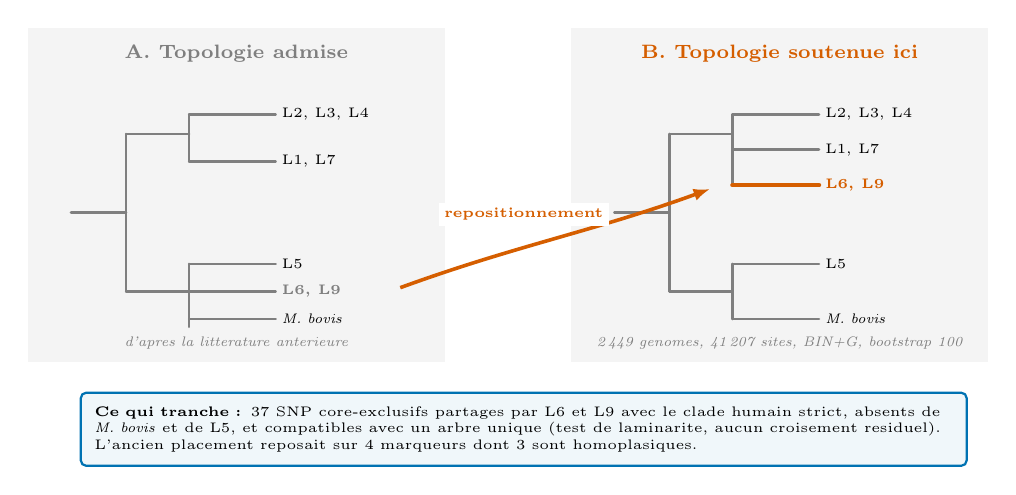
\begin{tikzpicture}[
    every node/.style={font=\scriptsize, align=center},
    br/.style={line width=0.9pt, color=oldgrey, cap=round},          % branche
    brnew/.style={line width=1.6pt, color=newred, cap=round},        % branche revisee
    tip/.style={font=\tiny, anchor=west, inner sep=1.5pt},
    tipnew/.style={tip, text=newred, font=\tiny\bfseries},
    hdr/.style={font=\scriptsize\bfseries, align=center},
    src/.style={font=\tiny\itshape, text=oldgrey, align=center},
    move/.style={-{Latex[length=6pt]}, line width=1.3pt, newred, shorten >=4pt, shorten <=4pt}
  ]

  % ============ PANNEAU A : la topologie admise ==========================
  \begin{scope}[xshift=0cm]
    \begin{scope}[on background layer]
      \fill[paneltint] (-0.55,-3.5) rectangle (4.75,0.75);
    \end{scope}
    \node[hdr, text=oldgrey] at (2.1,0.42) {A. Topologie admise};
    \node[src] at (2.1,-3.25) {d'apres la litterature anterieure};

    \draw[br] (0,-1.6) -- (0.7,-1.6);                       % racine
    \draw[br] (0.7,-0.6) -- (0.7,-2.6);                     % premier noeud
    \draw[br] (0.7,-0.6) -- (1.5,-0.6);                     % vers clade humain
    \draw[br] (0.7,-2.6) -- (1.5,-2.6);                     % vers clade animal

    \draw[br] (1.5,-0.35) -- (1.5,-0.95);
    \draw[br] (1.5,-0.35) -- (2.6,-0.35); \node[tip] at (2.62,-0.35) {L2, L3, L4};
    \draw[br] (1.5,-0.95) -- (2.6,-0.95); \node[tip] at (2.62,-0.95) {L1, L7};

    \draw[br] (1.5,-2.25) -- (1.5,-2.95);
    \draw[br] (1.5,-2.25) -- (2.6,-2.25); \node[tip] at (2.62,-2.25) {L5};
    \draw[br] (1.5,-2.95) -- (1.5,-3.05);
    \draw[br] (1.5,-2.60) -- (2.6,-2.60); \node[tip, text=oldgrey] at (2.62,-2.60) {\textbf{L6, L9}};
    \draw[br] (1.5,-2.95) -- (2.6,-2.95); \node[tip] at (2.62,-2.95) {\emph{M. bovis}};
  \end{scope}

  % ============ PANNEAU B : ce que montrent les donnees ==================
  \begin{scope}[xshift=6.9cm]
    \begin{scope}[on background layer]
      \fill[paneltint] (-0.55,-3.5) rectangle (4.75,0.75);
    \end{scope}
    \node[hdr, text=newred] at (2.1,0.42) {B. Topologie soutenue ici};
    \node[src] at (2.1,-3.25) {2\,449 genomes, 41\,207 sites, BIN+G, bootstrap 100};

    \draw[br] (0,-1.6) -- (0.7,-1.6);
    \draw[br] (0.7,-0.6) -- (0.7,-2.6);
    \draw[br] (0.7,-0.6) -- (1.5,-0.6);
    \draw[br] (0.7,-2.6) -- (1.5,-2.6);

    \draw[br] (1.5,-0.35) -- (1.5,-1.25);
    \draw[br] (1.5,-0.35) -- (2.6,-0.35); \node[tip] at (2.62,-0.35) {L2, L3, L4};
    \draw[br] (1.5,-0.80) -- (2.6,-0.80); \node[tip] at (2.62,-0.80) {L1, L7};
    \draw[brnew] (1.5,-1.25) -- (2.6,-1.25); \node[tipnew] at (2.62,-1.25) {L6, L9};

    \draw[br] (1.5,-2.25) -- (1.5,-2.95);
    \draw[br] (1.5,-2.25) -- (2.6,-2.25); \node[tip] at (2.62,-2.25) {L5};
    \draw[br] (1.5,-2.95) -- (2.6,-2.95); \node[tip] at (2.62,-2.95) {\emph{M. bovis}};
  \end{scope}

  % ============ le mouvement, explicite ==================================
  \draw[move] (4.05,-2.60) to[out=20,in=200] (6.9+1.35,-1.25);
  \node[font=\tiny\bfseries, text=newred, fill=white, inner sep=2pt]
    at (5.75,-1.62) {reposition\-nement};

  % Une figure avant/apres doit dire CE QUI TRANCHE, sinon elle n'est qu'un dessin
  % de deux opinions cote a cote.
  \node[draw=keepblue, thick, rounded corners=2pt, fill=keepblue!6, inner sep=5pt,
        text width=10.9cm, font=\tiny, align=left]
    at (5.75,-4.35)
    {\textbf{Ce qui tranche :} 37 SNP core-exclusifs partages par L6 et L9 avec le clade humain
     strict, absents de \emph{M.\ bovis} et de L5, et compatibles avec un arbre unique
     (test de laminarite, aucun croisement residuel). L'ancien placement reposait sur
     4 marqueurs dont 3 sont homoplasiques.};

\end{tikzpicture}
\end{document}
